% Setup - do not change
\documentclass[11pt]{article}
\usepackage[top=0.9in, left=0.9in, bottom=0.9in, right=0.9in]{geometry} 
\usepackage{parskip}

\usepackage[english]{babel}
\usepackage[utf8]{inputenc}
\usepackage{amsmath,amsthm,amssymb,graphicx,pdfpages,lipsum,hyperref}
\usepackage[none]{hyphenat}
\usepackage{csquotes}

\setlength\parindent{0pt}
%%%%%%%%%%%%%%%%%%%%%%%%%%%%%%%%%%%%%%%%%%%%%%%%%%%%%%%%%%%%%%%%%%%
% add other packages here if required
\usepackage{diagbox}
\usepackage{xcolor,colortbl}
\usepackage{subcaption}
%% Bibliography are specified in this file. You can also choose inline bib style if you want to. But make sure your citation style is consistent (and proper)
% For more details on citation: https://library.unimelb.edu.au/recite
\usepackage[sorting=none]{biblatex}

\addbibresource{references.bib}

%%%%%%%%%%%%%%%%%%%%%%%%%%%%%%%%%%%%%%%%%%%%%%%%%%%%%%%%%%%%%%%%%%% the '%' symbol denotes comments

% Begin document creation
% DELETE THE \lipsum PLACEHOLDERS WHEN YOU BEGIN
\title{\textbf{Predicting Tip Amount for Taxi Services in NYC}}
\author{
Shuran Zhang \\
Student ID: 1266122 \\
%% Replace the link with your github repo
% 1. Remember to escape underscore (\_) in the link.
% 2. Remember to include the commit you want to submit in the link
\href{https://github.com/MAST30034-Applied-Data-Science/mast30034-project-1-shuranzhang3}{Github repo with commit}
}

\begin{document}
\maketitle

\section{Introduction}
In 2020, the sudden outbreak of the COVID-19 pandemic led to a rapid increase in the number of confirmed cases. During this pivotal phase of pandemic containment, The U.S. Federal Government implemented strict home isolation measures, significantly suppressing the travel requirements of city dwellers. Consequently, the yellow taxi sector endure substantial immediate losses, experiencing a sharp and precipitous decline. Research indicates that throughout the pandemic, passenger numbers plummeted by 50\%, resulting in an alarming 80\% reduction in earnings for the majority of yellow taxi drivers \cite{ling2023}.

Taking on the viewpoint of a yellow taxi driver, this report aims to predict the tip amount for trips across different areas within New York City (NYC). The prediction process employs Linear Regression and Random Forest Regression models, utilizing input features to generate a comprehensive overview of the tip distribution landscape. This holistic understanding can then inform practical recommendations for yellow taxi drivers to optimize their earnings.

\subsection{Dataset}
The primary data set selected for this paper originates from the NYC Taxi \& Limousine Commission, specifically the TLC Taxi Trip Record Data. This data set encompasses trip details (such as pick-up and drop-off times and locations, tip amount, etc.) for all completed journeys using yellow taxis within NYC \cite{tlc}. The influence of travel limitations and the adverse effects stemming from the pandemic have waned since 2022. Hence, we opted to employ data spanning from January 2022 to December 2022 for our modelling and analysis, given its broader applicability to the yellow taxi market.

In addition to the existing taxi data set, we integrated external data sets, which encompass the dates of federal holidays in NYC for 2022 \cite{holiday} and a daily summary of weather reports from NYC Central Park provided by the US National Center for Environmental Information's (NCEI) Integrated Surface Data set \cite{weather}. From the collection of climate data set, various features, including average temperature and weather (such as snow, haze, etc.), will be used to furnish the models with a comprehensive depiction of the prevailing daily weather conditions. These external data sets are anticipated to exhibit non-negligible correlations with tip amounts in the context of yellow taxi services. 

\section{Preprocessing}
The data sets underwent a series of preprocessing steps to align them with the expected structure. The following section will outline the challenges identified in each data set and illuminate the approaches we undertook to address them. Throughout this section, our objective is to modify the data to enhance its suitability and precision for the purposes of modeling and analysis.

\subsection{Data Wrangling and Feature Selection}
\subsubsection{TLC Trip Record Data}
\begin{figure}[h]
    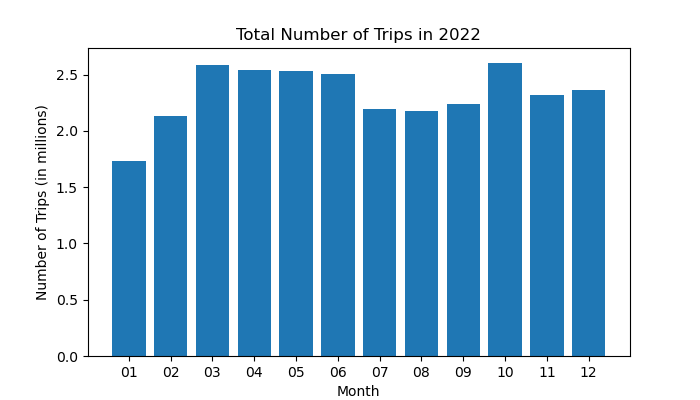
\includegraphics[width=0.7\textwidth]{plots/Number_of_Trips_WRT_Month_bar.png}
    \centering
    \caption{The number of yellow taxi trips taken between January 2022 and December 2022}
\end{figure}
Figure 1 reveals a notably even distribution of total trip numbers across month. A significant gap is noticeable between January and the other months due to a rapid surge in confirmed COVID-19 cases during the period \cite{covid}. Consequently, this observed gap is reasonable and well-founded.

Upon examining the raw taxi data set, which comprised 39,656,098 rows, we identified a number of issues within the data. These issues ranged from discrepancies that did not align with our research criteria to outright entry errors. This section will provide an overview of the various types of issues that were uncovered.

\begin{enumerate} 
    \item \textbf{Invalid records of passenger count} were included in some of the taxi data sets. A total of 763,344 instances with negative or zero passenger counts were identified and removed. Additionally, in accordance with NYC Transport regulations \cite{passenger}, considering the maximum capacity of 5 passengers for yellow taxis, another 457,191 instances were detected and removed.
    \item \textbf{Invalid records of trip distance} were included in some of the taxi data sets. A total of 574,059 instances with negative or zero trip distance were identified and removed.
    \item \textbf{Invalid records of trip dates} were included in some of the taxi data sets. A total of 476 instances with non-2022 trips were identified and removed.
    \item \textbf{Invalid records related to money} includes trips with negative tip amount, fare amount and total amount that are less than \$2.5. There are 448 instances with these records were detected and removed.
    \item \textbf{Invalid records for predicting tips} were determined by the payment type. Regarding to the description given by yellow taxi data dictionary from the NYC Taxi \& Limousine Commission, only credit card has tip amount records. Hence, there are 7,724,991 instances with non-credit payment were detected and removed.
    \item \textbf{Invalid records of pick-up/drop-off location ID} were those are out of the range 1-263, since they are recognized as undefined location. There are 453,126 instances with undefined location were detected and removed.
    \item \textbf{Outliers} were included in some of the taxi data sets. From research, the recommended tip amount should be 20\% of the fare amount \cite{tips}. Hence, we keep trip with tip proportion (this feature will mention in next section) within 0 and 0.5. Also, the average distance of yellow taxi is 300 km \cite{taxi}, so we remove unrealistic trip distance, such as 510 km. There were 479,658 instances were detected and removed.
    \item \textbf{Modifying data type} is required to improve our performance of model fitting. ``VendorID'' is a categorical feature with two values, so we changed it into boolean values. 
    \item \textbf{Invalid records with missing values} helps to maintain data integrity and ensure more accurate modeling and analysis. There are 556 instances with missing values were detected and removed.
\end{enumerate}

\subsubsection{NCEI Integrated Surface Data set}
The weather data set corresponds to distinct dates, with each row encompassing weather information for a particular day. Consequently, the emphasis of data wrangling for this data set resolves around transforming its attributes into formats conductive to our modeling objectives.
\begin{enumerate}
    \item \textbf{Discerning the magnitude of wind strength} provides us with a tangible understanding of the attribute ``AWND'' (average wind speed). The wind strength is defined as a ordinal feature with 5 feature values based on the Wind Scale of National Weather Service \cite{wind}. 
    \item \textbf{Computing average temperature}. From the data set, there majority data of ``TAVG'' are null. Hence, we used the maximum and minimum temperature to calculate the average temperature.
    \item \textbf{Replacing missing values}. Given that each row in this data set corresponds to a day, outright removal of rows with missing values is unfeasible. Consequently, our approach involves substituting missing values with ``0'' and considering those features in a boolean manner, such as ``snow'' and ``fog''.
\end{enumerate}
\subsubsection{Feature Engineering}
To enhance the performance of our models, we opted to incorporate additional features that could potentially exhibit correlations with tip amounts. For the yellow taxi data set, those features included: \\
\begin{enumerate}
    \item Adding a weekday/weekend boolean attribute (``weekend''), where 1 represents weekend.
    \item Adding a holiday attribute (``holiday'').
    \item Adding a tip proportion attribute (``tip\_prop''), calculated by tip amount divided by fare amount. 
    \item Extract different attributes from pick-up date-time, including pick-up year, pick-up month, and pick-up date.
    \item Extract useful features from weather data set to yellow taxi data set, including average temperature (``tavg''), wind strength (``wind\_strength''), ``snow'', ``thunder'', ``haze''.
\end{enumerate}

\section{Preliminary Analysis and Geo-spatial Visualisation}
Within this section, we conducted both individual explorations of the features with the yellow taxi data set and examined their connections with the weather data sets.
\subsection{Distribution of Tip-earning Proportion}
Our analysis uncovers a significant correlation between tip-related attributes (including tip amount and tip proportion) and location ID. Illustrated in Figure 2, the tip-earning proportion represents the average tip amount per trip, classified distinctly according to the identical location ID for both pick-up and drop-off points. In this figure, noticeable elevated tip-earning proportions are evident in regions like Staten Island (SINY) and the primary airports in NYC, namely Neward-Liberty (EWR), LaGuardia (LGA), and John F.Kennedy International (JFK). Regarding pick-up demand, heightened tip proportions are observed around the three airports, SINY, and Manhattan. Similarly, for drop-off demand, increased tip proportions are concentrated around SINY and EWR.
\begin{figure}[h]
    \centering
    \begin{subfigure}[t]{0.4\textwidth}
        \centering
        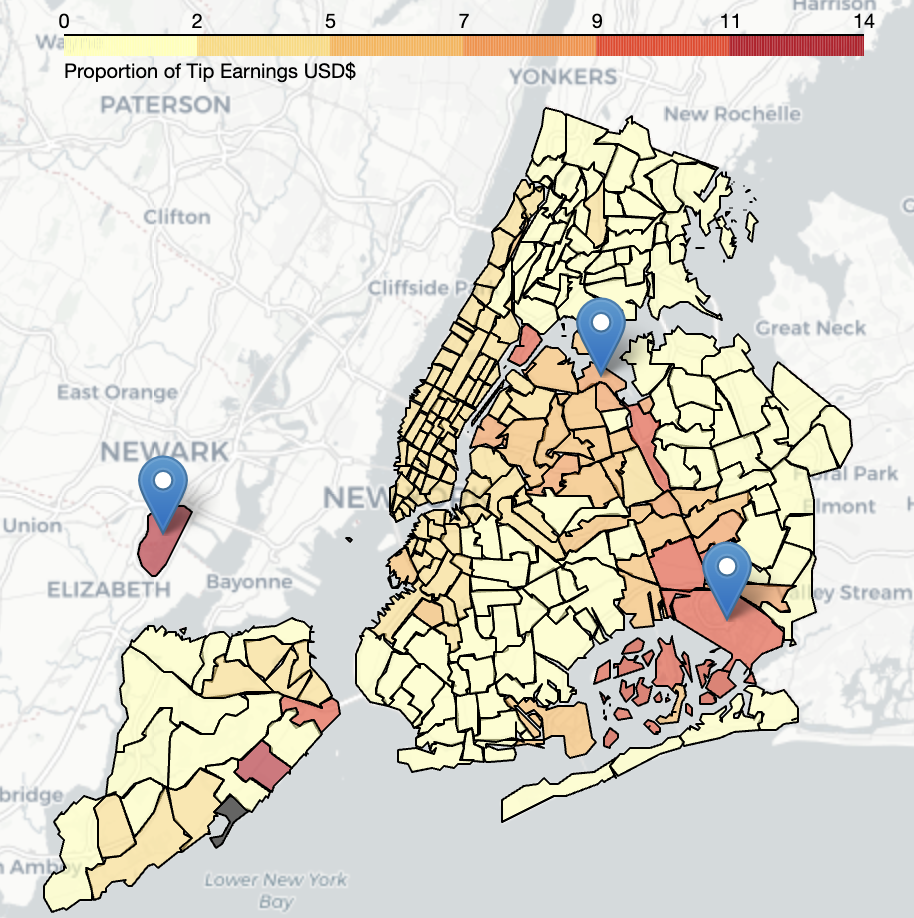
\includegraphics[width=.9\textwidth]{plots/tip_prop_pick.png}
        \caption{pick-up}
        \label{fig:pick-up}
    \end{subfigure}
    \begin{subfigure}[t]{0.4\textwidth}
        \centering
        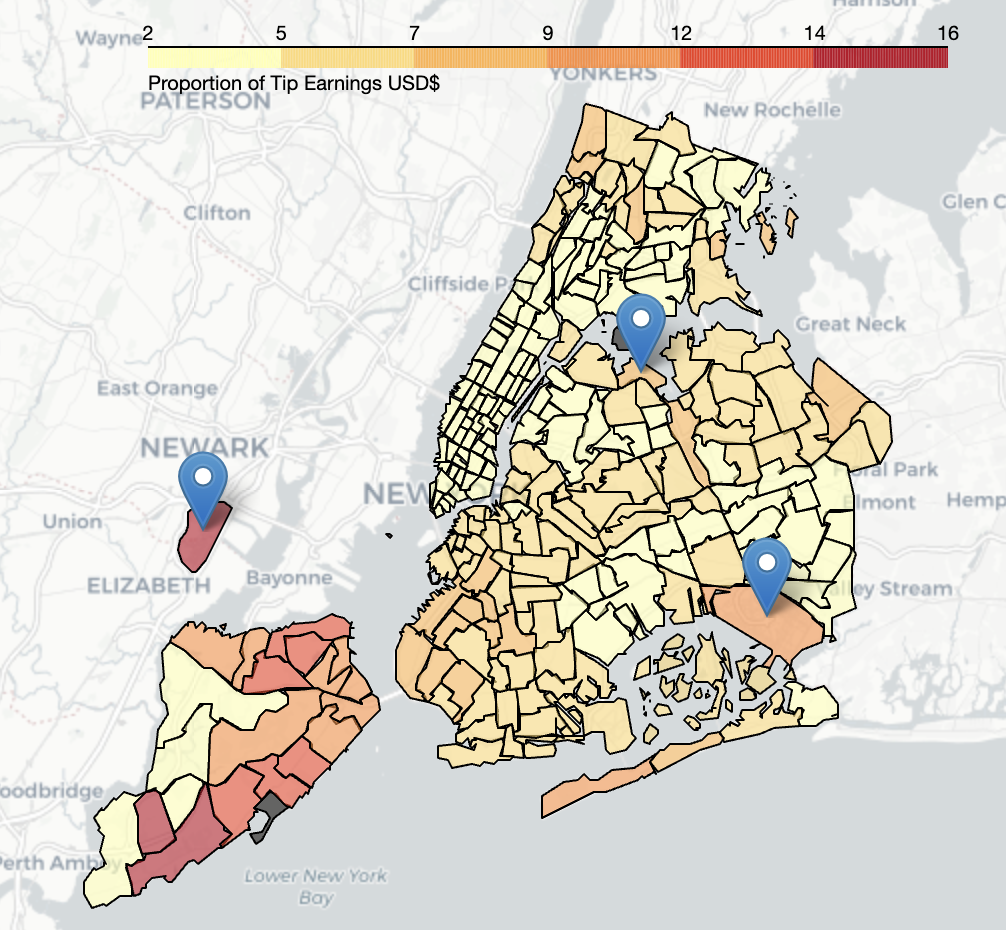
\includegraphics[width=1\textwidth]{plots/tip_prop_drop.png}
        \caption{drop-off}
        \label{fig:pick-up}
    \end{subfigure}
    \caption{Distribution of Tip-earnings Proportion in NYC}
\end{figure}
\subsection{Relationship between Tip Proportion and Other Predictors}
\begin{figure}[h!]
    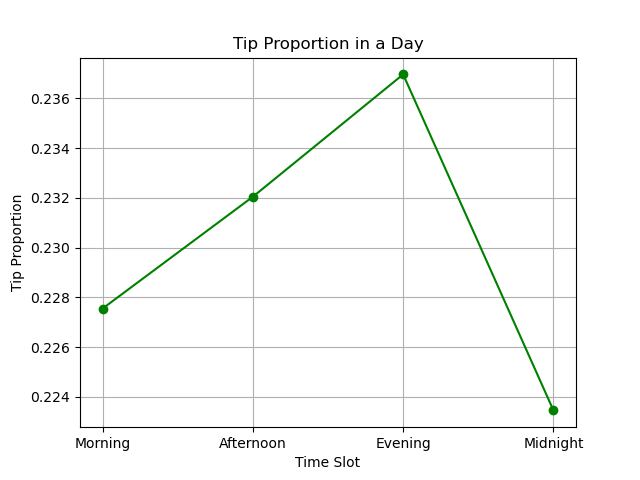
\includegraphics[width=0.53\textwidth]{plots/Tip_Proportion_WRT_Timeslot.png}
    \centering
    \caption{Tip Proportion VS Timeslot}  
\end{figure} 
Presented in Figure 3, the tip proportion signifies the average tip amount per dollar of fare amount. The graph accentuates that trips taking place during evening hours (6-10 pm) showcase the highest tip proportion, approximately 24\%. This occurrence can likely be attributed to the fact that the evening period coincides with a peak travel time for NYC citizens, as they conclude their workday or engage in nighttime activities and entertainment. In contrast, trips in the morning hours (6-11 am) and midnight hours (10 pm - 5 am) exhibit comparatively lower tip proportions, around 22.8\% and 21\%, respectively. The 22.8\% tip proportion during morning hours could be influenced by higher fare amounts due to extended travel times during the morning peak when citizens are heading to work. The lowest tip proportion during the midnight hour could potentially be explained by the general routines of NYC citizens during those hours.\\

With our analysis aiming to aid yellow taxi drivers in optimizing earnings, our focus naturally gravitates towards trips displaying relatively higher tip proportions. Examining Table 1, it becomes evident that weekdays and non-holidays exhibit elevated tip proportions, standing at 26.09\% and 25.91\%, respectively. The heightened tip proportion during weekdays can be attributed to various factors, including the higher column of business-related travel and the activity of business districts (e.g., Manhattan) inhabited by high-income professionals. Passengers hailing from these locales may be more inclined to extend larger tips. 
\begin{table}[h!]
    \centering
    \begin{tabular}{|c|c|c|c|c|c|} \hline
    \diagbox{Day Type}{Time Slot} & Morning & Afternoon & Evening & Midnight\\ \hline\hline
    Weekday & 24.93\% & 25.41\% & \cellcolor{blue!23}26.09\% & 24.67\%\\ \hline
    Weekend & 25.12\% & 25.15\% & 25.42\% & 24.67\%\\ \hline 
    Non-holiday & 24.97\% & 25.34\% & \cellcolor{blue!23}25.91\% & 24.67\%\\ \hline
    Holiday & 25.21\% & 25.09\% & 25.35\% & 24.57\%\\ \hline
    No Snow & 24.97\% & 25.32\% & 25.88\% & 24.65\%\\ \hline
    Snow & 25.38\% & 25.88\% & \cellcolor{blue!23}26.42\% & 25.57\%\\ \hline
    No Thunder & 24.99\% & 25.34\% & 25.89\% & 24.67\%\\ \hline
    Thunder & 24.87\% & 25.28\% & \cellcolor{blue!23}25.90\% & 24.58\%\\ \hline
    No Haze & 24.98\% & 25.33\% & 25.89\% & 24.65\%\\ \hline
    Haze & 24.97\% & 25.38\% & \cellcolor{blue!23}25.94\% & 24.77\%\\ \hline
\end{tabular}
\caption{Tip Proportion Throughout Different Day Types and Time Slots}
\end{table}
Conversely, the diminished tip proportion on holidays might stem from individuals dedicating time to connect with family and friends, resulting in a shift away from conventional tipping behaviours. Moreover, holiday periods could introduce a change in passenger demographics, with an influx of tourists and less-frequent travelers who might not be as familiar with local tipping norms. This shifting demographic can impact overall tipping trends. 

In the context of weather conditions, instances of extreme weather, such as snow, thunder, and haze, correlate with amplified tip proportions. This can be attributed to passengers acknowledging the taxi driver's exceptional efforts in navigating adverse conditions. Furthermore, extreme weather often heightens travel inconvenience and discomfort, prompting passengers to display gratitude through larger tips as a gesture of appreciation for the taxi driver's role in providing convenience and comfort despite challenging circumstances. 

\section{Modelling}
Within this section, we employed two distinct regression models, specifically Linear Regression and Random Forest Regression, to assess their effectiveness in predicting tip amounts for taxi trips in NYC. In pursuit of capturing the generalized relationship between predictors and response, our approach involved utilizing two months from each season for training the model, while employing the remaining months as the evaluation data set for testing purposes. The response variable is tip amount, and the predictors are the other features, such as fare amount, trip distance, and wind strength.
\subsection{Linear Regression (LR)}
In preparation for Linear Regression, it was necessary to transform categorical predictors into continuous ones by converting their data types to integers or floats. Additionally, a choice was made to carefully select the predictors employed for model training, aiming to prevent excessive model complexity. This lead to the creation of a correlation matrix for analysis. As depicted in Figure 4, it indicates that both fare amount and total amount share robust correlations with the tip amount. Nevertheless, it is crucial to acknowledge that fare amount and total amount are also highly correlated. Consequently, the decision was made to exclude total amount as a predictor, considering the desire to mitigate issues stemming from multicollinearity. 
\begin{figure}[h]
    \centering
    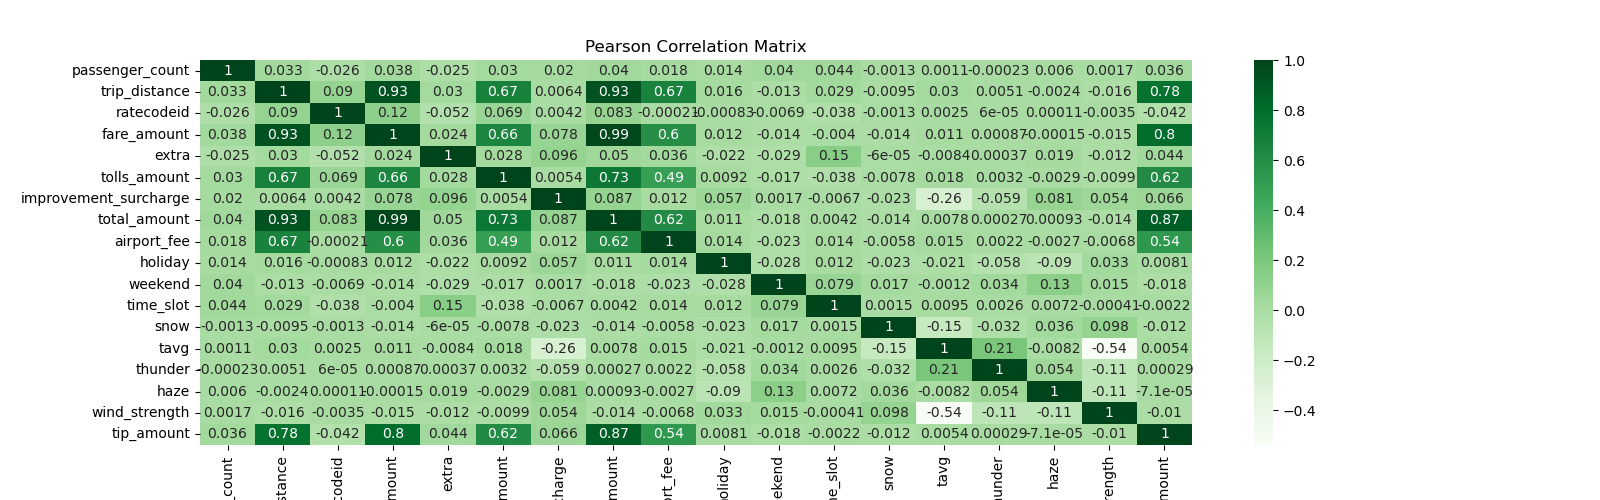
\includegraphics[width=1.32\textwidth]{plots/Pearson_Correlation_Matrix.png}
    \caption{Pearson Correlation Matrix}  
\end{figure} 
Subsequent to this, we operated under the assumption of no interactions between the remaining predictors within the linear model. As a result, the model we employed can be expressed as follows:
\begin{equation}
    Y_{ij} = \beta_0 + \sum_{j=1}^{p}(\beta_{ij} X_{ij}) + \epsilon_{ij}
\end{equation}\\
where $\beta_0$ is the intercept, $p$ is the number of predictors, $\beta_{ij}$ is the effect for the $j^{th}$ predictor.
\subsection{Random Forest Regression (RFR)}
Random Forest Regression introduces randomness in the selection of subsets of training attributes and features. This addresses the issue of decision trees being prone to overfitting. Additionally, each random tree's training process is independent of the others and occurs concurrently, saving considerable computational time in model training. Consequently, Random Forest Regression is generally recognized for its robust performance.Given the relatively ample size of our training data set, we have set the maximum depth of this model to 10, thereby preventing kernel interruptions stemming from excessive workload.

\section{Results and Discussion}
To assess and compare the performance of the Linear Regression and Random Forest Regression models, we utilized the mean squared error (MSE) as our evaluation metric. MSE measures the average of squared differences between the predicted tip amount and the actual tip amount within the data set. This offers a numerical gauge of the extent to which the predictions from the regression models correlate with the actual values.\\
\begin{table}[h]
\centering
\begin{tabular}{|c|c|}\hline
& MSE\\ \hline\hline
Linear Regression & 2.64\\ \hline
Random Forest Regression & 2.55\\ \hline
\end{tabular}
\caption{Mean Squared Error of the Models}
\end{table}\\
From table 2, we can observe that the Random Forest Regression model has a lower MSE, indicating enhanced accuracy in predicting tip amounts. To thoroughly assess the models' performance, we generated a geo-spatial visualization that illustrates the difference between the actual and predicted tip amounts.
\begin{figure}[h]
    \subfloat[LR]{
    \begin{minipage}[t]{0.45\linewidth}
    \centering
    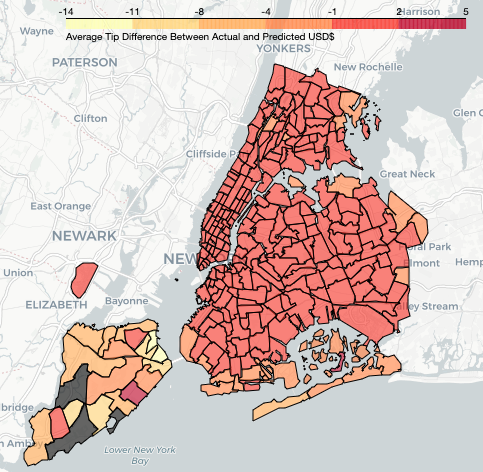
\includegraphics[width=2.5in]{plots/tip_diff_lm.png}
    \end{minipage}}
    \subfloat[RFR]{
    \begin{minipage}[t]{0.45\linewidth}
    \centering
    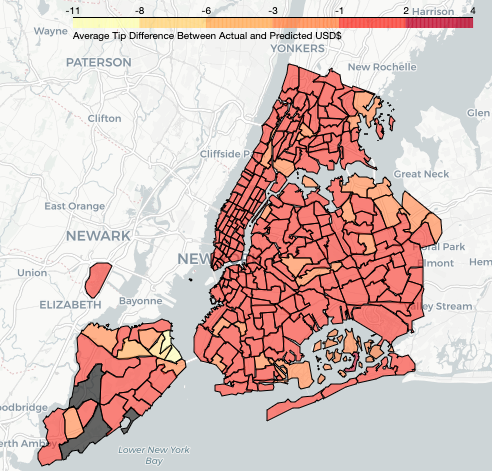
\includegraphics[width=2.5in]{plots/tip_diff_rf.png}
    \end{minipage}}
    \caption{Distribution of Difference in Actual and Predicted Tip Amounts in NYC}
\end{figure}\\
As shown in Figure 5, the statistical metric employed is the average difference between the actual and predicted tip amounts for each trip at the corresponding pick-up location ID. It is notable that the majority of absolute differences between actual and predicted tip amounts from both models predominantly fall within the \$1-2 range. However, the Linear Regression model tends to overestimate tip amounts for tips originating at SINY, shown by larger orange area. In contrast, the Random Forest Regression model yields comparatively smaller differences for the same pick-up location. Consequently, the Random Forest Regression model results in a lower MSE value. This geographic visualization underscores the efficacy of the Random Forest Regression model in accurately predicting tip amounts for yellow taxi trips in NYC.

\section{Recommendations}
Based on our assessment of the models, it is evident that the Random Forest Regression model excels in estimating tip amounts for yellow taxi rides in NYC, showcasing a narrower gap between actual and predicted tip amounts.

For the companies in the taxi industry, we recommend them to employ their internal data sets to develop and refine predictive models similar to the ones analyzed in the study. This can empower drivers with accurate tip forecasts, optimizing their route choices and earning potential. Also, they can offer training sessions to the taxi drivers about leveraging tip prediction tools effectively to help them understand the significance of strategic pick-ups and timings to maximize their earnings. This will further motivate drivers by offering a clearer earning outlook, which resulting in a win-win situation for both companies and employed drivers. 

For taxi drivers, we propose prioritizing passenger pick-ups around high-tip-earning locations, particularly SINY and major airports like EWR, LGA, and JFK, since these areas are likely to yield better tips depicted in Figure 2. Additionally, focusing on evening shifts (6-10 pm), particularly on weekdays or non-holidays. Moreover, during days with extreme weather conditions such as snow. thunder, or haze, seize the opportunity to pick up more passengers while ensuring safety drive. As previous analysis in Section 3, passengers might recognize and appreciate the efforts of taxi drivers navigating through challenging circumstances. 

\section{Conclusion}
This report delved into the analysis and forecasting of tip amounts for yellow taxi services in New York City. Leveraging visualizations, we gained enhanced understanding of tip proportions across trips. We examined and assessed two distinct regression models for predicting tip amounts using historical taxi trip data. The integration of external data sets, including official holiday dates and daily weather data, enriched our regression models, yielding promising outcomes. To achieve even more precise tip amount predictions, we could incorporate more comprehensive external data, such as per capita income based on the same location ID.
\clearpage

% BEGIN REFERENCES SECTION
\printbibliography
\end{document}
